\section{Lokale Modelle}
Für das Ausführen von Modellen zum Testen werden in dieser Arbeit zwei Techniken angewandt. Zum einen mittels Ollama Framework, das mit einer Web-GUI erweitert werden kann, zum anderen durch Dateien, welche beispielsweise mit dem Python Framework Langchain abgefragt werden können.\vspace{0.2cm}

Die Modelle werden auf einem Debian 12 Server mit 32 GB RAM und einem 16 Kernprozessor ausgeführt. Um große Modelle zu testen wurde mit einer Swap-Partition von 100 GB gearbeitet, um die Ausführung größerer Modelle zu ermöglichen.\vspace{0.2cm}

\subsection{Modellbereitstellung mit Ollama}
Für das Testen der lokalen Modelle wird das Ollama Framework angewandt. Dies ermöglicht eine neben einer Benutzeroberfläche im Browser eine Anbindung an einer API. Diese lässt sich beispielsweise mittels Python abfragen. Auf dieser Weise lassen sich Modelle von der \href{https://ollama.com/search}{Ollama Modell} Seite testen. Dazu wird Ollama auf dem Server installiert und konfiguriert, siehe Anhang \ref{sec:install_config_ollama_local}. Nach dem Download stehen die Modelle zur Verfügung und es können Interaktionen mit dem Modell erfolgen.\vspace{0.2cm}

Zusätzlich kann ein grafisches Tool zum Testen installiert werden. Mit deren Hilfe können die Modelle leicht getestet werden. Mit Open WebUI wird ein Browser basierendes Toll eingesetzt, dass auf dem Ollama-Server installiert wird. Nach der Installation ist das Tool einsatzbereit und im lokalen Netzwerk, unter http://<<server-ip>>:<<webui-port>> erreichbar. Die Installation wird im Anhang \ref{sec:open_webui} beschrieben.


\subsection{Modellbereitstellung als Datei}
Eine zweite Methode zur Bereitstellung von Modellen die für diese Arbeit Verwendung findet, ist die direkte Nutzung als lokale Datei. Diese können dann direkt angesprochen werden, in dieser Arbeit wird Python verwendet. Hierbei wurden die Modelle von Hugging Face fokussiert. Diese lassen sich unter anderem mit dem Python Framework \href{https://pypi.org/project/langchain/}{Longchain} orchestrieren.\vspace{0.2cm}

Nachdem die Modelle von Hugging Face heruntergeladen und lokal abgespeichert wurden, sind diese ohne größeren Aufwand anwendbar. Ein Beispiel für ein mögliches Download-Skript ist in Anhang \ref{sec:hugging_face_models} im Listing \ref{lst:download_hugging_face_model_by_cache} und \ref{lst:download_hugging_face_model} zu sehen. Hierbei ist zu beachten das genügend freier RAM zur Verfügung steht, um die Modelle abzuspeichern.

%-------------------------------------------------------------------------------------------


%\subsection{Orchestrierung von Modellen}
%Die Orchestrierung der Modelle erfolgt mithilfe des Python-Frameworks Longchain. Hierbei werden an die Modelle verschiedene Anforderungen gestellt. Zum einen müssen die Modelle Code generieren, zum anderen ist die Anforderung Text zu erstellen oder zu überarbeiten. Die Abbildung \ref{img:orchestration_llms} zeigt schematisch den Aufbau der orchestrierten Modelle. Der Textfilter sucht in der Ausgabe des ersten Modells den Prompt und eliminiert die Anweisungen und Erklärungen.

%\begin{figure}[!ht]
%	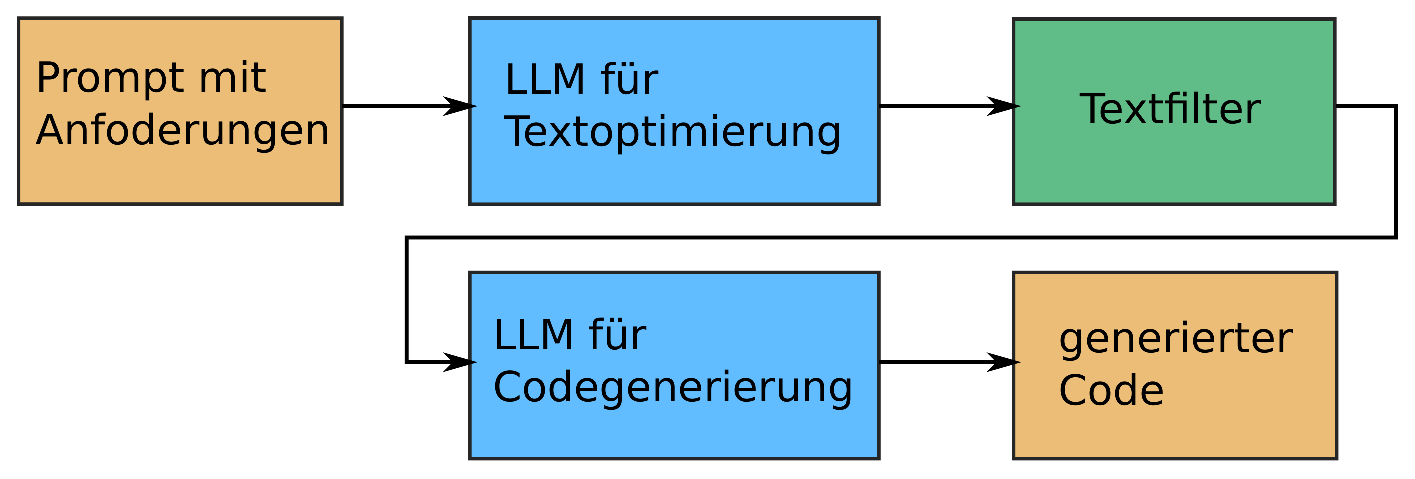
\includegraphics[width=0.8\textwidth]{content/chapter_implementation/images/orchestrierung_llms.eps}
%	\centering
%	\caption{Orchestrierte LLM's für die Codegenerierung}
%	\label{img:orchestration_llms}
%\end{figure}

%-------------------------------------------------------------------------------------------


%\section{Online Modelle}
%Text.

\section{Benchmark Codeevaluation}\label{sec:benchmark_evaluation}
Ausführen des Benchmarks.


\subsection{Problemabfragen an die Modelle}
Nachdem die Modelle bereitstehen, erfolgt Erstellung der Antworten von den Modellen. Mit Prompts welche die Probleme aus dem HumanEval-XL Benchmark enthalten, werden nun die Modelle abgefragt. Die vollständigen Antworten werden, für eine spätere Auswertung als JSONL-Dateiformat gespeichert. Für jedes Problem erfolgen zehn Abfragen an jedes Modell. Für die Evaluierung der lokalen Modelle wurden sowohl Modelle von Hugging Face als auch Modelle von Ollama verwendet, siehe Kapitel \ref{subsec:llm_selection} für die Zuordnung der Modelle.

\subsection{Auswertung der Modellantworten}
Die Auswertung der Antworten wird für jedes Modell angepasst, da die Antworten von Modell zu Modell variieren. Hier werden unterschiedliche Möglichkeiten für Codesnippets angewendet, beispielsweise (\texttt{```php}) oder (\texttt{```php \textbackslash n <?php}), welche für die Ausführung anzupassen sind. Somit wird immer nur die Methode zur Extrahierung des Codes aus den Antworten geändert, siehe Beispielcode im Listing \ref{lst:evaluation_search_generated_code}.\vspace{0.2cm}

Mit den vorliegenden Codesnippets und den Tests aus dem jeweiligen Problem, wird ein ausführbarer PHP-Code erstellt und mittel Python ausgeführt. Die Tests werfen Exceptions, wenn der Code die Anforderungen nicht erfüllt oder Laufzeitfehler auftreten. Dann gibt der Code als nicht verwertbar. Der Code \ref{lst:php_interpreter_in_python} zeigt den Ausschnitt im Code zur Ausführung des PHP Interpreters.

\begin{lstlisting}[
language=Python,
caption={Codesnippet zur Ausführung des PHP Interpreters}
label=lst:php_interpreter_in_python
]
for answer in answers:
    answer = answer.replace(r"\n", "\n")
    try:
        result = subprocess.run(
            ["php", "-r", f"{test}{answer}"],
            capture_output=True,
            text=True,
            check=False,
            timeout=5,
        )
    except subprocess.TimeoutExpired:
        pass

    if result.stderr.strip() == "":
        answer_result_fault = True
\end{lstlisting}

Die unbehandelte Execption führt lediglich dazu, dass die Programmausführung nicht unterbrochen wird. Der hier abgefangene Timeout wird in der nachfolgenden \texttt{if} Klausel behandelt. Aus den erhaltenen Ergebnissen, berechnet die \texttt{pass@k} Metrik die Zuverlässigkeit des jeweiligen vorgegebenen Problems, hinsichtlich Codegenerierung. Des Weiteren wird anschließend der Durchschnitt für die Zuverlässigkeit des Modells errechnet.\vspace{0.2cm}

\textbf{Umsetzung der pass@k Metric}\vspace{0.2cm}

In Python steht, hierfür die Bibliothek \textit{pass\_at\_k} zur Verfügung. Der PHP Code wurde auf einen Debian 11 mit PHP in der Version 8.2.26 evaluiert.

\begin{lstlisting}[language=Python,label=lst:pass_at_k,caption={Berechnung der pass@k Metrik in Python}]
def custom_pass_at_k(n: int, c: int, k: int) -> float:
    """
    :param n (int): numbers of total samples.
    :param c (int): number of currect samples.
    :param k (int): number of consider samples.
    """
    if n - c < k:
        return 1.0
    return 1.0 - np.prod(1.0 - k / np.arange(n - c + 1, n + 1))
\end{lstlisting}


\section{Codeevaluation mit Frameworks}
Neben dem bekannten Evaluationen mit beispielsweise dem HumanEval Benchmark, wird hier eine weitere Testmethodik überprüft, die mit verschiedenen Validierungstools der jeweiligen Programmiersprache ausgeführt wird. Für die Erstellung der Abfragen wird das Python-Skript verwendet, was schon im Kapitel \ref{sec:benchmark_evaluation} vorgestellt wurde.

\subsection{PHP Codeevaluation}
Der Test wird bei den erweiterten Problemen durchgeführt und beginnt mit den Unit-Tests die mit \textit{PHPUnit} durchgeführt werden. Im Anschluss wird \textit{PHPMetrics} ausgeführt. Hierbei wird geprüft, ob die Codekomplexität und Wartbarkeit überprüft. Sind diese Tests bestanden, wird der Code noch gegen eine \textit{SonarQube} Server validiert. Die Ausführung der Tests wird mithilfe eines Python-Skripts durchgeführt. Es wird eine PHP Datei erstellt, die mit den Frameworks geprüft wird.

\subsection{JavaScript Codeevaluation}
Text.

%\section{Online Modelle}
% Eigenen KI Server \href{https://www.computerweekly.com/de/ratgeber/Einen-KI-Server-mit-Ollama-und-Open-WebUI-einrichte}{Computer Weekly}
% Orchestrierung mit Python \href{https://pypi.org/project/multillm/}{multillm-Projekt}
% LangChain Library \href{https://python.langchain.com/api_reference/ollama/chat_models/langchain_ollama.chat_models.ChatOllama.html}{Example}
% \href{https://pypi.org/project/langchain-ollama/}{Python lib langchain-ollama}
% YouTube \href{https://www.youtube.com/@AICodeKing}{AICodeKing}
